\begin{usecase}{Extract Events from WhatsApp}
  \ucbasicinfo{High}{Regular}
  \ucshortdescription{System monitors WhatsApp messages of connected WhatsApp accounts and extracts event details using Large Language Models (LLMs), adding them to the user's calendar.}
  \uctrigger{A message is sent to the connected WhatsApp account of an arbitrary user in our system.}
  \ucactors{WhatsApp}{}
  \ucpreconditions{At least one WhatsApp account must be connected.}
  \ucrelationships{Suggest Conflict Resolution}{N/A}{N/A}
  \ucinputsoutputs{
    \begin{itemize}
      \item \textbf{Messages sent to currently selected user} (Source: WhatsApp)
      \item \textbf{Context window of last 15 messages} (Source: WhatsApp)
    \end{itemize}
  }{
    \begin{itemize}
      \item \textbf{Extracted event details in JSON format} (Destination: System)
      \item \textbf{Push notification to user} (Destination: User's Device)
    \end{itemize}
  }
  \ucmainflow{
    \begin{enumerate}
      \item A sent message is received and the user has replied and 30 seconds have passed without any interruptions.
            \ucinfo{System reads the last 15 messages to establish conversation context.}
      \item The conversation context is sent to the LLM service with a carefully engineered prompt.
            \ucinfo{The prompt instructs the LLM to analyze messages for event details (date, time, location), consider context, and return structured JSON output while handling various date/time formats.}
      \item The LLM processes the context and returns event details if found.
            \ucinfo{The system validates the extracted information and prepares it for calendar insertion.}
      \item Add the detected event to the user's calendar.
            \ucinfo{System notifies user via push notification about the newly added event.}
    \end{enumerate}
  }
  \ucalternateflows{
    \begin{itemize}
      \item If there is a conflict adding this event, send a notification telling the user that there is a conflict they need to resolve.
    \end{itemize}
  }
  \ucexceptions{
    \begin{itemize}
      \item If there is an error during extraction of events, fail silently and log it to a specific table in the database for debugging later by developers.
    \end{itemize}
  }
  \ucconclusion{System successfully adds the event to the user's calendar and notifies the user of the added event.}
  \ucpostconditions{The event is added to the user's calendar.}
  \ucbusinessrules{
    \begin{itemize}
      \item Only messages with events and its surrounding context shall be analyzed.
      \item System must wait for user's reply before analyzing the messages.
      \item System must wait for 30 seconds before initiating the analysis on messages after the user replies and reset as long the conversation is onggoing.
      \item The LLM prompt must be engineered to identify potential events, extract key details, and handle various conversation patterns.
    \end{itemize}
  }
  \ucspecialrequirements{
    \begin{itemize}
      \item The system must have access to the user's WhatsApp account as a client to receive and read messages.
      \item The LLM service must be configured to handle natural language processing of informal conversations.
    \end{itemize}
  }
\end{usecase}

The ``Extract Events from WhatsApp Sequence Diagram'', shown in \textbf{Figure~\ref{fig:seq/extract-events-whatsapp}}, illustrates the automated event extraction process from WhatsApp conversations. The system operates in a continuous monitoring loop where the WhatsApp Service (implemented using whatsapp-web.js) listens for incoming messages. Upon receiving a message, the service implements a 30-second delay to gather conversation context, collecting the last 15 messages from the chat history to ensure comprehensive event detection.

The gathered context is then forwarded to the Backend, which interfaces with the LLM Service using a specialized prompt engineered for event detection. This prompt is specifically designed to:
\begin{itemize}
  \item Identify potential events within informal conversations
  \item Extract crucial details including date, time, and location
  \item Process various date and time formats
  \item Generate structured JSON output for system processing
\end{itemize}

\begin{figure}[!h]
  \centering
  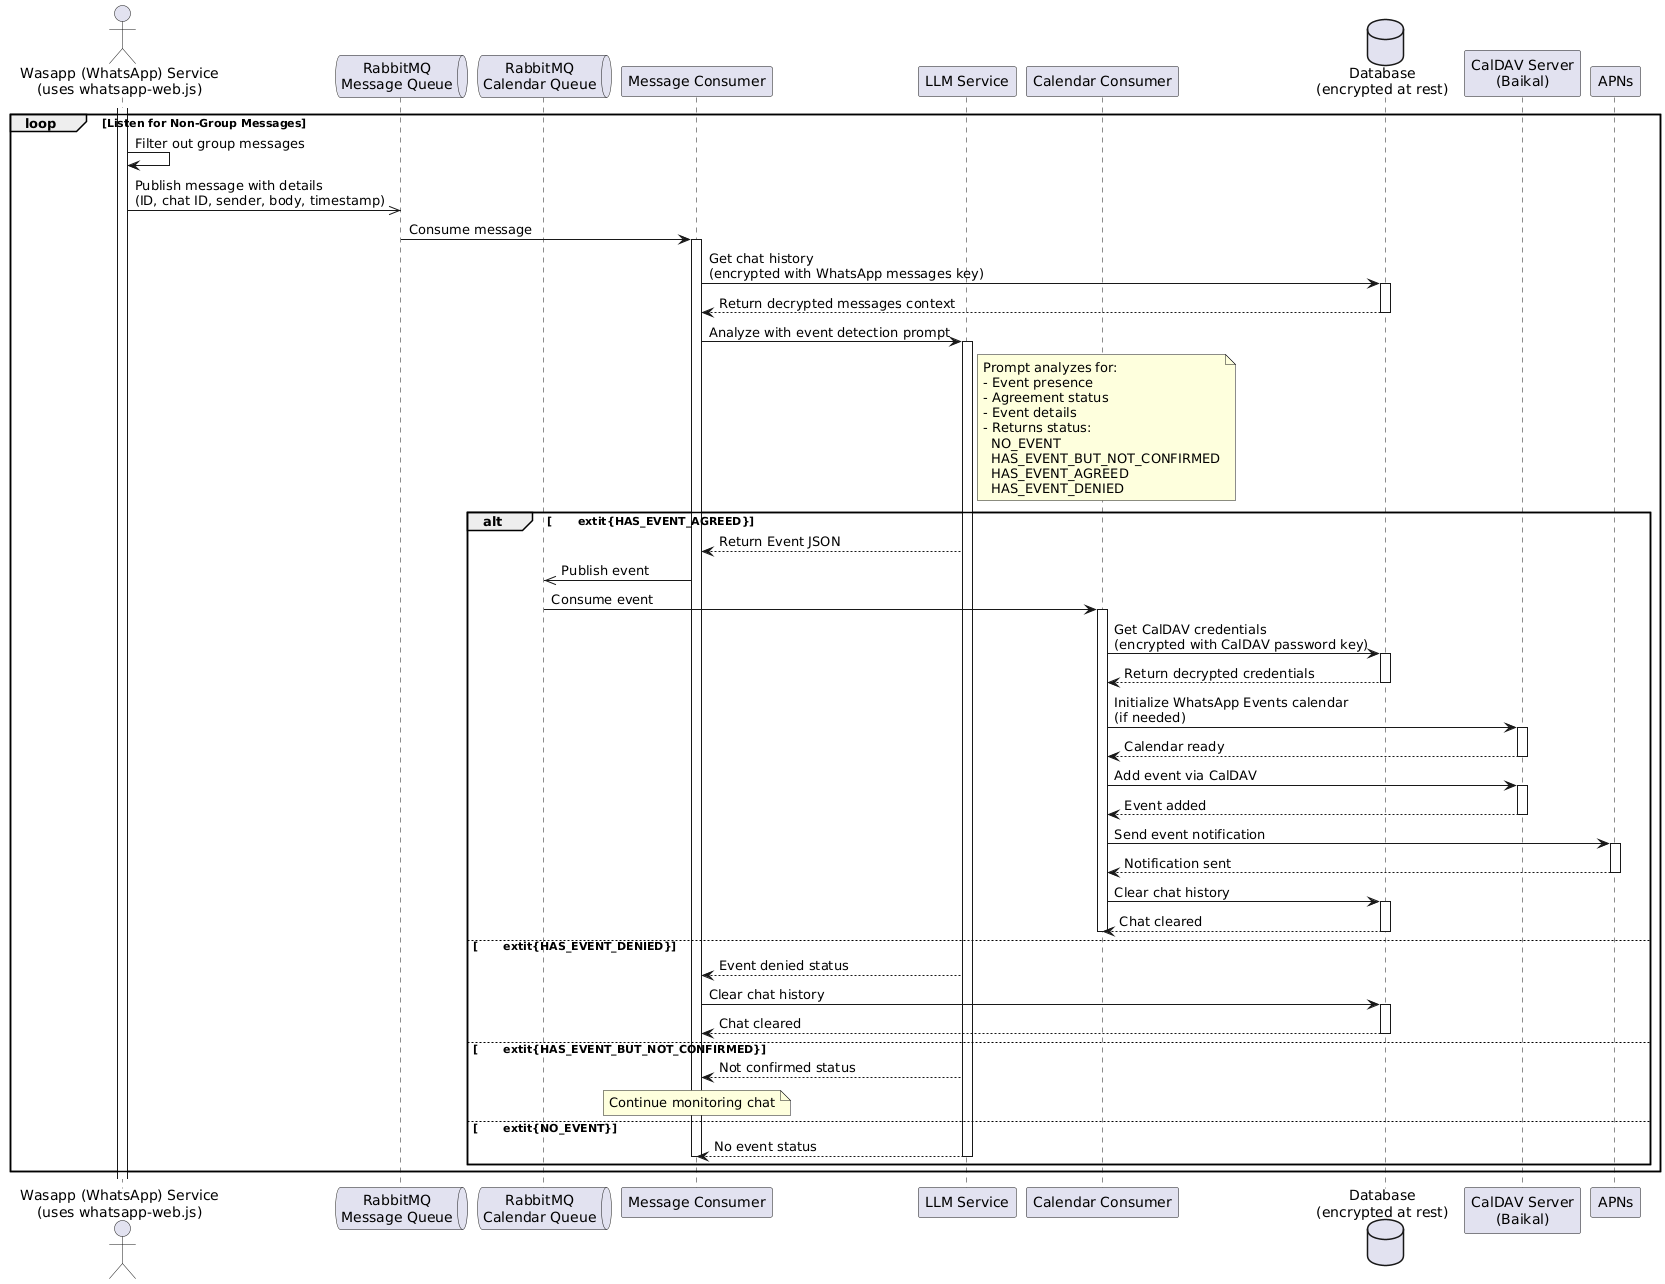
\includegraphics[width=\textwidth]{images/docs/diagrams/sequence-diagrams/all-sequence-diagrams/Extract Events from WhatsApp.png}
  \caption{Extract Events from WhatsApp Sequence Diagram}
  \label{fig:seq/extract-events-whatsapp}
\end{figure}

When the LLM Service detects an event, it returns a structured JSON response to the Backend. The Backend then:
\begin{enumerate}
  \item Validates the extracted event information for accuracy
  \item Stores the validated event in the Database
  \item Retrieves the relevant Device IDs for the event owner
  \item Triggers a push notification through Apple's Push Notification service (APNs)
\end{enumerate}

If no event is detected in the analyzed context, the system silently continues its monitoring loop without user notification. This automated workflow ensures efficient event capture from natural conversations while maintaining user awareness through targeted notifications. The system's ability to understand context and process informal language patterns makes it particularly effective for extracting event details from casual WhatsApp conversations.